 \documentclass[oneside,a4paper,12pt]{pictreport}
\usepackage{dirtree}
\usepackage{enumitem}
\usepackage{amsmath}
\usepackage{listings}

%\usepackage[table,xcdraw]{xcolor}
\usepackage{graphicx}
\usepackage[ruled,vlined,linesnumbered]{algorithm2e}
\usepackage{multirow}
\usepackage{enumitem}
\setlist[enumerate]{itemsep=0mm}


\lstset{basicstyle=\ttfamily,
  showstringspaces=false,
  commentstyle=\color{red},
  keywordstyle=\color{blue}
}
%\usepackage{showframe}
%\hoffset = 8.9436619718309859154929577464789pt
%\voffset = 13.028169014084507042253521126761pt
\usepackage{enumitem}
\setlist{parsep=0pt,listparindent=\parindent} %


\fancypagestyle{plain}{%
  \fancyhf{}
  \fancyfoot[C]{PICT, Department of Computer Engineering, 2017}
  \fancyfoot[R]{\thepage}
}
\pagestyle{fancy}
\fancyhead{}
\renewcommand{\headrulewidth}{0pt}
\footskip = 0.625in
\cfoot{}
\rfoot{}

\usepackage[hidelinks]{hyperref}
\usepackage{tikz}
\usetikzlibrary{arrows,shapes,snakes,automata,backgrounds,petri}

\usepackage{tabularx}

\usepackage[nottoc,notlot,notlof,numbib]{tocbibind}
\usepackage[titletoc]{appendix}
\usepackage{titletoc}
\renewcommand{\appendixname}{Annexure}
\renewcommand{\bibname}{REFERENCES}

\setcounter{secnumdepth}{5}
\usepackage{float}
\usepackage{subcaption}
\usepackage{multirow}

\usepackage[ruled,vlined]{algorithm2e}

\begin{document}

\picttitlepage{SENTIMENT ANALYSIS USING ORIGINAL AND REVERSED REVIEWS}{Kaushik S. Hande}{6989}{Prof. A. G. Phakatkar}

%\companycertificate{BEHAVIORAL ASSESSMENT OF INTERNAL AND EXTERNAL CANDIDATES OF MULTIPLE ORGANIZATIONS USING SENTIMENT ANALYSIS AND EMOTION MINING}{Sagar S. Patil}{}{Mr. Vijay Kumbhar}{Mr. Vijay Kumbhar}{}

\pictcertificate{SENTIMENT ANALYSIS USING ORIGINAL AND REVERSED REVIEWS}{Kaushik S. Hande}{6989}{Prof. A. G. Phakatkar}{}





\setcounter{page}{0}
\frontmatter
\cfoot{PICT, Department of Computer Engineering, 2017}
\rfoot{\thepage}
\pagenumbering{Roman}
\pictack{SENTIMENT ANALYSIS USING ORIGINAL AND REVERSED REVIEWS}{Kaushik S. Hande}{}{}

\listoffigures 
\listoftables
		
\begin{pictabstract}
Bag of words (BOW) is used for modeling in machine learning algorithms. 
However, BOW is not able to handle negation well
because of its fundamental deficiencies. Many ways are used
to handle the problem of negation which results into polarity
shift. They require either knowledge about language constructs
or extra human interventions which eventually increases the
complexity. In this work, a data expansion technique, called dual
sentiment analysis (DSA), is used to address the polarity shift
problem due to negation in sentiment classification. Both original and
reversed reviews are used to classify the test reviews in dual sentiment 
analysis.

\end{pictabstract}



% \maketitle
\tableofcontents
\mainmatter



\titleformat{\chapter}[display]
{\fontsize{16}{15}\filcenter}
{\vspace*{\fill} \bfseries\LARGE\MakeUppercase{\chaptertitlename}~\thechapter}
{1pc}
{\bfseries\LARGE\MakeUppercase}
[\thispagestyle{empty}\vspace*{\fill}\newpage]





\setlength{\parindent}{11mm}
\chapter{SYNOPSIS}


\section{Dissertation Title}
Sentiment Analysis using Original and Reversed Reviews.

%\section{Sponsorship}
%Webonise Lab, Pune.

%\section{External Guide} 
%Mr. Vijay Kumbhar

\section{Internal Guide}
Prof. A. G. Phakatkar



\section{Problem Statement}
\label{sec:problem_def}
`` To make use of the original and reversed review samples in pairs for training a
statistical classifier and make predictions. ''

\section{Objectives}
\begin{itemize}

    \item To train the classifiers using reviews and actual labels.
    \item To obtain the predictions of labels (positive review or negative review) for test data.
    \item To use opposite reviews to correctly classify the review class.
\end{itemize}

\section{Hypothesis}

Polarity shift causes accuracy of classifier to decrease. We assume that 
original review and corresponding opposite review can be used together to increase the accuracy of 
review class label prediction and to avoid the problem caused due to polarity shift.

\section{Relevant Mathematics Associated with Dissertation}

\subsection{Mathematical Model}

%\begin{equation*}
$S=\{s,e,I,O,fmain|\phi\}$\\ 
%\end{equation*}
where,\\
s = start state\\
e = end state\\
I = Inputs to the system\\
I = \{x,x${'}$,y,$y{'}$,D,D${'}$\}\\
where,\\
x = original sample\\
x${'}$ = reversed sample\\
y $\in$ \{0,1\} = The class label of the original sample\\
y${'}$ = \(1-y\) = The class label of the reversed sample\\
$
D = {(x_i,y_i )}_{i=1}^{n}$ = original training set\\
$ D{'}= {(x_i{'},y_i{'} )}_{i=1}^{n}$ = The reversed training set\\
O = Output \\
O = \{ p(x),p(x${'}$),p(x,x${'}$)\}\\
where\\
p(x) = Prediction for the original sample\\
p(x${'}$) = Prediction for the reversed sample\\
p(x,x${'}$) = Dual prediction based on a pair of sample\\
$f_{main} =\{f_{reverse},f_{classifier}\}$\\
$f_{reverse} =$ function for reversing the corresponding each review\\
$f_{classifier} =$ classifier for the prediction of class of review


\subsection{Metrics for Performance Evaluation}
The parameters helpful to evaluate performance of supervised
machine learning algorithm is based on the element from a matrix 
known as confusion matrix or contingency table. It is used
in supervised machine learning algorithm to help in assessing
performance of any algorithm. From classification point of view,
terms such as ``True Positive(TP)'', ``False Positive (FP)'', ``True 
Negative(TN)'', ``False Negative (FP)'' are used to compare label of classes
in this matrix as shown. True Positive represents the number of reviews those are
positive and also classified as positive by the classifier, where as
False Positive indicates positive reviews, but classifier does not
classify it as positive. Similarly, True Negative represents 
the reviews which are negative also classified as negative by the 
classifier, where as False Negative are negative reviews but classifier
does not classify it as negative.

\par Based on the values obtained from confusion matrix, other 
parameters such as ``precision'', ``recall'', ``f-measure'', and ``accuracy''
are found out for evaluating performance of any classifier.


\begin{itemize}
\item \textbf{Precision} : It measures the exactness of the classifier result. It is
the ratio of number of examples correctly labeled as positive to
total number of positively classified example.
\begin{equation}
\frac{TP}{TP + FP}
\end{equation}
\item \textbf{Recall} : It measures the completeness of the classifier result. It is
the ratio of total number of positively labeled example to total
examples which are truly positive.
\begin{equation}
\frac{TP}{TP + FN}
\end{equation}
\item \textbf{F-Measure}: It is the harmonic mean of precision and recall. It
is required to optimize the system towards either precision or recall, which 
have more influence on final result.
\begin{equation}
\frac{2 \times Precision \times Recall}{Precision + Recall}
\end{equation}
\item \textbf{Accuracy} : It is the most common measure of classification 
process. It can be calculated as the ratio of correctly classified 
example to total number of examples. 
\begin{equation}
\frac{TP + TN}{TP + TN + FP + FN}
\end{equation}
\end{itemize}

\chapter{TECHNICAL KEYWORDS}
\section{Area of Dissertation}
Natural language processing, machine learning, sentiment analysis, opinion mining.

\section{ACM Keywords}
\begin{enumerate}[label=\Alph*]
    \item Information Systems
    \begin{enumerate}[label*=.\arabic*]
    \item Information Retrievals
    \begin{enumerate}[label*=.\arabic*]
        \item Retrieval tasks and goals
        \begin{enumerate}[label*=.\arabic*]
            \item Sentiment analysis
            \item Clustering and classification
        \end{enumerate}
        \end{enumerate}
    \end{enumerate}
    \item Computing methodologies
        \begin{enumerate}[label*=.\arabic*]
            
            \item Machine learning
            \begin{enumerate}[label*=.\arabic*]
                \item Supervised learning by classification
                \begin{enumerate}[label*=.\arabic*]
                    \item Multinomial Naive Bayes
                    \item Random Forest
                    \item Support Vector Machines
                \end{enumerate}
            \end{enumerate}
        \end{enumerate}
    \end{enumerate}
\chapter{INTRODUCTION}

\section{Dissertation Idea}

\par Sentiment is an attitude, thought, or judgement prompted by feeling. Sentiment analysis 
is also known as opinion mining, it involves studing of people’s sentiments towards 
certain entities. Internet is a resourceful place with respect to sentiment information. From a
perspective of a user, people are able to express their views through various social media,
such as forums, micro-blogs, or online social networking sites \cite{pang2008}.

\par With the advent of web 2.0 techniques,
users started prefering to share their opinions on the Web. These user-generated and 
sentiment-rich data are valuable to many applications like 
credibility analysis of news sites on the web, recommendation system, business and 
government intelligence etc. At the same time, it brings
urgent need for detecting overall sentiment inclinations of
documents generated by users, which can be treated as a
classification problem. Sentiment analysis includes several
subtasks which have seen a great deal of attention in recent years:
\begin{enumerate}
 \item To detect whether a given document is subjective or objective.
  \item To identify whether given subjective document express a positive opinion or a negative opinion.
  \item To determine the sentiment strength of a document,
such as strongly negative, weakly negative, neutral, weakly
positive and strongly positive.
\end{enumerate}

In this work we are focusing on second subtask.

\par Besides individuals on social media marketers also need to monitor all media for information related to their brands
whether it's for public relations activities, fraud violations, or competitive intelligence.
Thus, aside from individuals, sentiment analysis is also the need of companies which are anxious to understand how
their products and services are perceived by the public.

\par The dominating text representation method in
both supervised and 
semi supervised sentiment
classification is known as the bag-of-words (BOW)
model \cite{pang}, which is difficult to meet the requirements
for understanding the review text and dealing with
complex linguistic structures such as negation. For
example, the BOW representations of two opposite
reviews `` It works well'' and `` It doesn't work well''
are considered to be very similar by most statistical
learning algorithms \cite{yahoo}.The two sentiment opposite texts are considered to be very similar by the
BOW representation. This is exactly why standard machine learning algorithms often
fail under the circumstance of polarity shift due to negation in the sentences of the review text \cite{contrast} \cite{xiaOriginal}.

\par Several approaches have been proposed in the literature
to address the polarity shift problem .They require either knowledge about language constructs or
extra human interventions which eventually increases the complexity in classification of sentiment.  Such
high-level dependency on external resources makes the systems 
difficult to be widely used in practice. There were also
some efforts to address the polarity shift problem with the
absence of extra annotations and linguistic knowledge. However, results are still far from satisfactory.
\section{Motivation of Dissertation}
Polarity shift is a kind of linguistic phenomenon which can reverse the sentiment polarity of the text. Negation is
the most important type of polarity shift \cite{xiaOriginal}. For example, by adding a negation word ``don't'' to a positive text ``I like
this book '' in front of the word ``like'', the sentiment of the
text will be reversed from positive to negative. However, the two sentiment-opposite texts are considered to be
very similar by the BOW representation. This is the main reason why standard machine learning algorithms often
fail under the circumstance of polarity shift.


\chapter{LITERATURE SURVEY}

We studied the related work on sentiment analysis and
polarity shift.

\section{Sentiment Analysis and Polarity Shift}
\hspace{1.1cm}According to the levels of granularity, tasks in sentiment
analysis can be divided into four categorizations: document-
level, sentence-level, phrase-level, and aspect-level sentiment analysis.
\par 
For document and sentence-level sentiment classification, 
there are two main types of methods in the literature:
term-counting and machine learning methods \cite{yahoo} \cite{pang} \cite{pang2008} \cite{ruiEnssemble}. In 
term-counting methods, the overall orientation of a text is
obtained by summing up the orientation scores of content
words in the text, based on manually-collected or external
lexical resources \cite{turney} \cite{turney1}. In machine learning methods,
sentiment classification is regarded as a statistical 
classification problem, where a text is represented by a 
bag-of-words; then, the supervised machine learning algorithms
are applied as classifier \cite{pang}. Accordingly, 
the way to handle polarity shift also differs in the two types of methods.
\par
The term-counting methods can be easily modified to
include polarity shift. One common way is to directly
reverse the sentiment of polarity-shifted words, and then
sum up the sentiment score word by word \cite{valence}. Compared with term counting methods, the machine
learning methods are more widely discussed in the 
sentiment classification literatures. However, it is relatively
hard to integrate the polarity shift information into the
BOW model in such methods. For example, Das and
Chen \cite{yahoo} proposed a method by simply attaching ``NOT``
to words in the scope of negation, so that in the text ``I
don't like this book'', the word ``like'' becomes a new word ``like-NOT''.
Yet Pang et al. \cite{pang} reported that this method only
has slightly negligible effects on improving the sentiment
classification accuracy.
\newpage




\section{Gap Identification Through Literature Survey}

The following table shows the literature survey about different techniques of sentiment analysis used for classification. 

\renewcommand{\arraystretch}{1.0}
\begin{center}
\begin{table}[h!]
\caption{Literature Survey} 
\begin{tabular}{|l|l|l|l|}
\hline
No. & Reference                                                              & Techniques                                                                & Description                                                                 \\
\hline
1   & \begin{tabular}[c]{@{}l@{}}Dual Sentiment Analysis:\\ Considering Two sides of \\ 
one review \cite{xiaOriginal} \end{tabular}
  & \begin{tabular}[c]{@{}l@{}}Support vector machine\\(SVM), Naive bayes,\\ Logistic Regression \end{tabular}   
         & \begin{tabular}[c]{@{}l@{}}Dual training and \\
Dual Prediction \\technique is used.\end{tabular}                                                                                                                                                                                         \\
\hline
2   & \begin{tabular}[c]{@{}l@{}}Thumbs up? Sentiment \\
Classification using\\
Machine learning\\
algorithms \cite{pang} \end{tabular} 
 & \begin{tabular}[c]{@{}l@{}}Learning algorithms\\
and n-gram model\end{tabular}                      
            & \begin{tabular}[c]{@{}l@{}}Classify the dataset\\
using different\\
machine.\end{tabular}                                                                                                                                                                      \\
\hline
3   & \begin{tabular}[c]{@{}l@{}}Classification of \\sentiment
reviews using\\
N-gram machine \\learning
approach \cite{base} \end{tabular}                 & \begin{tabular}[c]{@{}l@{}}Support Vector Machine\\
Naive Bayes \end{tabular}            & \begin{tabular}[c]{@{}l@{}}Converting text\\
reviews into numeric\\
matrices using\\
countvectorizer and\\
TF-IDF\end{tabular}                                                                                                                                                          \\
\hline
4   & \begin{tabular}[c]{@{}l@{}}Thumbs up or \\thumbs
down? Semantic \\orientation
applied to \\unsupervised
classification \\of reviews \cite{turney}\end{tabular}                                          & \begin{tabular}[c]{@{}l@{}}Unsupervised
learning \\algorithm for\\
classifying a \\review\end{tabular}                                                         & \begin{tabular}[c]{@{}l@{}}A specific unsupervised\\
learning technique \\based
on the\\
mutual information\end{tabular}                                                                                                                                                                                        \\
\hline
5   & \begin{tabular}[c]{@{}l@{}}Automatic Opinion \\polarity
Classification \\of movie \cite{salvetti}\end{tabular} & \begin{tabular}[c]{@{}l@{}}Naive Bayes\\
And Markov Model \\(MM) \end{tabular}  & \begin{tabular}[c]{@{}l@{}} Accessed overall \\opinion
polarity(OVOP)\\
concept using \\machine
learning\\ algorithm\end{tabular}                                                                                                                                                 \\
\hline
6   & \begin{tabular}[c]{@{}l@{}}Dual Training and \\dual
prediction for\\ polarity
classification \cite{xia} \end{tabular}                                                                                    & \begin{tabular}[c]{@{}l@{}} SVM and Naive Bayes\end{tabular}                                                           & \begin{tabular}[c]{@{}l@{}}Dual training and\\
dual prediction\\(DTDP)\end{tabular}                                                                                                                                                                          \\
\hline

\end{tabular}
\caption{Literature Survey} 
\end{table}
\end{center}


\chapter{PROBLEM DEFINITION AND SCOPE}

\section{Goals}
\begin{itemize}
\item Understanding existing sentiment analysis approaches.
\item Study corpus based, lexical based and semantic based techniques.
\item Understanding unigram, bigram, trigram and combination of them for modeling purpose.
\item Training the model with naive bayes, support vector machine, maximum entropy.
\item Applying this learned model to the test dataset.
\item Evaluating the results generated by classifiers.
\end{itemize}

\section{Objectives}

Please refer Chapter 1, Section 1.7 on Page 2

\section{Statement of Scope}
\begin{itemize}
\item Preprocessing the reviews.
\item Classify reviews into two polarities.
\item Evaluate the classification accuracy by each classifier.
\end{itemize}

\section{Software Context}
\subsection{Scikit-learn} 
Scikit-learn (formerly scikits.learn) is a free software machine learning library for the 
python programming language. It features various classification, regression and clustering
algorithms including support vector machines, random forests, gradient boosting,
k-means and DBSCAN, and is designed to interoperate with the Python numerical and scientific libraries NumPy and SciPy.

\subsection{NumPy}


NumPy is the fundamental package for scientific computing with Python. It contains among other things:
\begin{itemize}
\item A powerful N-dimensional array object
\item Sophisticated (broadcasting) functions
\item Tools for integrating C/C++ and Fortran code
\item Useful linear algebra, Fourier transform, and random number capabilities
\end{itemize}
Besides its obvious scientific uses, NumPy can also be used as
an efficient multi-dimensional container of generic data.
Arbitrary data-types can be defined. This allows NumPy to
seamlessly and speedily integrate with a wide variety of databases.

\subsection{Natural language toolkit (NLTK)}
NLTK is a leading platform for building Python programs to work with
human language data. It provides easy-to-use interfaces to over 50 corpora 
and lexical resources such as WordNet, along with a suite of text processing 
libraries for classification, tokenization, stemming, tagging, parsing, and 
semantic reasoning, wrappers for industrial-strength NLP libraries, and an active discussion forum.

\subsection{Matplotlib}
Matplotlib is a python 2D plotting library which produces publication 
quality figures in a variety of hardcopy formats and interactive environments 
across platforms. Matplotlib can be used in python scripts, the Python and IPython 
shell, the jupyter notebook, web application servers, and four graphical user interface 
toolkits. You can generate plots, histograms, power spectra, bar 
charts, errorcharts, scatterplots, etc., with just a few lines of code.

\chapter{DISSERTATION PLAN}

\section{Purpose of the Document}
This document specifies and estimates various risks
associated with this project and states how they are handled. 
It also states the project plan in terms of task and their dependency.

\section{Technical Constraints}
\begin{itemize}

\item Review size must be big enough for the classifier to predict.
A review of length 20-30 words or above is good for the classifier.
\end{itemize}

\section{Dissertation Estimates}
\subsection{Reconciled Estimates}
\subsubsection{Cost Estimates}
No cost is required for tools and software as open source softwares are used.
\subsubsection{Time Estimates}
Calendar time required: 11 months.
\subsubsection{Dissertation Resources}
\begin{itemize}

\item Software resources used are mentioned in Chapter 7, Section 7.5.1 on Page 26
\item Hardware resources used are mentioned in Chapter 7, Section 7.5.2 on Page 26

\end{itemize}

\section{Risk Management}
This section discusses dissertation risks and the approach to manage them.
\subsection{Risk Identification}
For risks identification, review of scope document, requirement 
specifications and schedule is done. Answers to questionnaire revealed 
some risks. Following risk identification questionnaire has been referred.
\begin{itemize}
\item Are requirements fully understood by the software engineering team and its customers?
\item Have customers been involved fully in the definition of requirements?
\item Do end-users have realistic expectations?
\item Does the software engineering team have the right mix of skills?
\item Are project requirements stable?
\item Is the number of people on the project team adequate to do the job?
\item Do all customer/user constituencies agree on the importance of the project 
and on the requirements for the system/product to be built?
\end{itemize}

\subsection{Risk Analysis}
The risks for the dissertation are analyzed within the constraints of time and quality. Risk can be as follows:

\begin{itemize}
\item Out of memory error, while creating model and training the model.
\item Review text contains unrecognized characters.
\item Out of memory error, while predicting on the test dataset.
\end{itemize}
Please refer Table 6.1, 6.2 and 6.3 for detail description.

\renewcommand{\arraystretch}{1.5}
\begin{table}[h!]
\caption{Risk Table}
\begin{tabular}{|l|l|l|l|l|l|}
\hline
\textbf{ID} & \textbf{Risk Description} & \textbf{Probability} & \multicolumn{3}{c|}{\textbf{Impact}}                                         \\ \hline
            & \textbf{}                 & \textbf{}            & \textbf{Schedule} & \textbf{Quality} & \textbf{Overall} \\ \hline
1           & Out of Memory             & High                & Low                      & High                    & High                    \\ \hline
2           & Unrecognized characters            & Low               & Medium                   & High                    & Medium                  \\ \hline
3           & Out of Memory         & Low               & Medium                   & High                    & High                    \\ \hline
\end{tabular}
\end{table}

\begin{table}[h!]
\centering
\caption{Risk Probability Definitions}
\begin{tabular}{|l|l|l|}
\hline
\textbf{Probability} & \textbf{Value}                   & \textbf{Description} \\ \hline
High                 & Probability of the occurrence is & \textgreater 75\%    \\ \hline
Medium               & Probability of the occurrence is & 26\% - 74\%          \\ \hline
Low                  & Probability of the occurrence is & 25\%                 \\ \hline
\end{tabular}
\end{table}

\begin{table}[h!]
\centering
\caption{Risk Impact Definitions}
\begin{tabular}{|l|l|l|}
\hline
\textbf{Impact} & \textbf{Value}    & \textbf{Description}                                                                                                                                        \\ \hline
Very High       & \textgreater 10\% & Schedule impact or unacceptable quality                                                                                                                     \\ \hline
High            & 5\%-10\%          & \begin{tabular}[c]{@{}l@{}} Schedule impact or some parts of \\ the project have low quality  \end{tabular}                                                                                              \\ \hline
Low             & \textless5\%      & \begin{tabular}[c]{@{}l@{}}Schedule impact or barely noticeable \\degradation in quality low impact on schedule or\\ quality can be incorporated\end{tabular} \\ \hline
\end{tabular}
\end{table}

\subsection{Overview of Risk Mitigation, Monitoring and Management}
Please refer Table 6.4, 6.5 and 6.6 for detail description.

\begin{table}[h!]
\centering
\caption{Risk 1}
\label{my-label}
\begin{tabular}{|l|l|}
\hline
\textbf{Risk ID}          & 1                                                    \\ \hline
\textbf{Risk Description} & Out of memory error, when training model \\ \hline
\textbf{Category}         & Configuration                                        \\ \hline
\textbf{Source}           & Software Requirement Specification Document          \\ \hline
\textbf{Probability}      & High                                                 \\ \hline
\textbf{Impact}           & High                                                 \\ \hline
\textbf{Response}         & Mitigate                                             \\ \hline
\textbf{Strategy}         & Changing number of features resolves this issue.     \\ \hline
\textbf{Risk Status}      & Occurred and Resolved                                \\ \hline
\end{tabular}
\end{table}


\begin{table}[h!]
\centering
\caption{Risk 2}
\label{my-label}
\begin{tabular}{|l|l|}
\hline
\textbf{Risk ID}          & 2                                                                     \\ \hline
\textbf{Risk Description} & Unreconized characters                                     \\ \hline
\textbf{Category}         & Configuration                                                         \\ \hline
\textbf{Source}           & Software Requirement Specification Document                           \\ \hline
\textbf{Probability}      & Low                                                               \\ \hline
\textbf{Impact}           & Low                                                                \\ \hline
\textbf{Response}         & Mitigate                                                              \\ \hline
\textbf{Strategy}         & Convert all characters into unicode format \\ \hline
\textbf{Risk Status}      & Occurred and Resolved                                                 \\ \hline
\end{tabular}
\end{table}
\begin{table}[h!]
\centering
\caption{Risk 3}
\label{my-label}
\begin{tabular}{|l|l|}
\hline
\textbf{Risk ID}          & 3                                           \\ \hline
\textbf{Risk Description} & Out of memory error, when predicting    \\ \hline
\textbf{Category}         & Development Environment                     \\ \hline
\textbf{Source}           & Software Requirement Specification Document \\ \hline
\textbf{Probability}      & Low                                     \\ \hline
\textbf{Impact}           & Low                                        \\ \hline
\textbf{Response}         & Mitigate                                    \\ \hline
\textbf{Strategy}         & Using sparse matrix to represent text                \\ \hline
\textbf{Risk Status}      & Occurred and Resolved                       \\ \hline
\end{tabular}
\end{table}
\newpage
\section{Staff Organization}

\subsection{Team Structure}
\begin{itemize}
    \item Internal Guide : Prof. A. G. Phakatkar
    %\item External Guide : Mr. Vijay Kumbhar
    \item Student : Kaushik S. Hande 
\end{itemize}

\subsection{Management Reporting and Communication}
The progress of dissertation is reported once in a month.
\subsection{Dissertation Task Set}


Major tasks in the Dissertation stages are - 
	
				
				\noindent Task 1 : Requirement
					\begin{enumerate}
						\item Define problem statement
						\item Identify scope, requirements
						\item Related mathematical model
					\end{enumerate}
				Task 2 : Design
					\begin{enumerate}
						\item Identifying of key objects, functional relation
						\item UML diagrams and functional dependency graph
						\item System design
					\end{enumerate}
				Task 3 : Implementation
				\begin{enumerate}
						\item Import dataset
						\item Classifier implementation
						\item Comparison using graphs
					\end{enumerate}
				Task 4 : Testing
					\begin{enumerate}
						\item Unit testing
						\item Integration testing
						\item System testing
					\end{enumerate}
				Task 5 : Integration and Maintenance
					\begin{enumerate}
						\item Integration
						\item Maintenance
					\end{enumerate}


\par Please refer figure 6.1 Task Network.
\newpage
\subsection{Task Network}
\begin{figure}[!h]
\centering
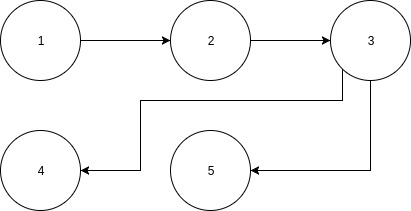
\includegraphics[width=3.7in,height=2.2in]{task.jpg}
\caption{Task Network}
\end{figure}
\newpage
\subsection{Timeline Chart}
Please refer Annexure B, Table B.1 on Page 61 for all Dissertation Tasks.
\vspace{5mm}
\begin{figure}[!h]
\centering
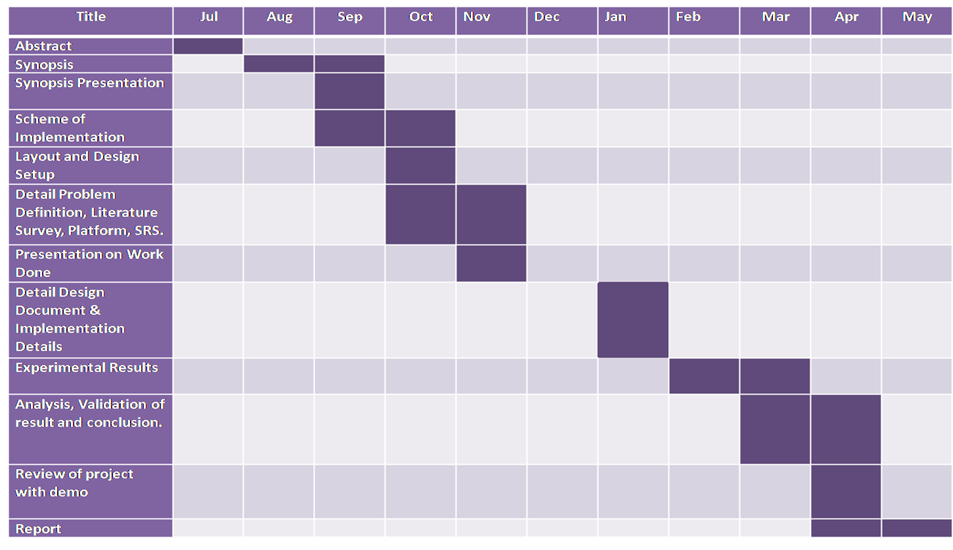
\includegraphics[width=5.5in,height=5.5in]{timeline.png}
\caption{Timeline Chart}
\end{figure}

\chapter{SOFTWARE REQUIREMENT SPECIFICATION}

\section{Introduction}
The aim of this document is to specify the software requirements for classification of movie reviews.

\section{Purpose and Scope of the Document}
The purpose of the document is to enlist various software requirements to build the system. This document has functional and non-functional requirements for the software being developed.

\section{Overview of Responsibilities of Developer}
The responsibilities of a developer includes gathering of information about the classification libraries, that can be used to design and develop the system to categorize movie reviews. The developer’s responsibilities include: 
\begin{itemize}
\item Planning for dissertation (Scheduling) 
\item Designing of system (High Level Design Document)
\item Coding of system (Implementation)
\item Testing of system (Test Cases)
\end{itemize}

\section{Product Overview}
System builds classifier models for classification of reviews. Different functionality of the system are : 

\begin{itemize}
\item Review loader : It loads the reviews into python environment.
\item Stopwords remover : It removes the stopwords like is, a, an, the, was, were etc.
\item Vectorizer : It converts the reviews into matrix of rows and columns where columns represents the words
and rows represents each reviews. Presence of particular word in a review is shown by the values in the columns.
\item Classifier : It classifies the reviews into positive and negative review.
\end{itemize}
\section{Hardware Resources Used}
\subsection{Software Requirements}
\begin{itemize}
				\item Python 2.7.6 
				\item Rstudio Version 0.99.893 
				\item R version 3.3.2
				\item Operating Systems:
					\begin{itemize}
						
						\item Ubuntu 14.04, Ubuntu 16.04
						
					\end{itemize}
\end{itemize}
\subsection{Hardware Requirements}
			\begin{itemize}
				\item Intel\textsuperscript{\textregistered} Core\textsuperscript{\texttrademark} i7-4790 CPU @ 3.60GHz x 8 , width : 64 bits
				\item Memory : 8 GB DDR3 or more
				\item Capacity : 1697MHz or more
				\item Cores : 8 or more
				\item PCI Express Gigabit Ethernet Controller, Size: 100Mbit/s, Capacity: 1Gbit/s, Width: 64 bits
				\item Hard Disk : 500 GB (EXT4 Primary/Logical Partition)
			\end{itemize}
		
\newpage

\section{Functionality}
\begin{itemize}
\item Download movie reviews from IMDB dataset.
\item Import the movie review dataset into python environment using csv package.

\item Convert the text reviews into matrix form.
\item Remove the stopwords from reviews.
\item Show positive and negative polarity score for test reviews.


\item Compare classifiers for accuracy of classification.
\end{itemize} 

\section{Input}
\begin{itemize}
\item Dataset that consists of movie reviews and their corresponding labels.
\item List of stopwords which play no role in classification.
\end{itemize}


\section{Output}
\begin{itemize}
\item Classification of each test review into positive or negative.
\item Confusion matrix of classification test data.
\item Percentage of accuracy achieved in classification.
\item Comparison of accuracies obtained by each classifier.
\end{itemize}

\section{Major Constraints}

\begin{itemize}
\item To store movie reviews as input in csv file format.
\item To execute classifiers in configured environment.
\item To train the model for polarity classification.
\end{itemize}

\section{Applications}
\begin{itemize}
\item Businesses and organisations which require consumer opinions to do with products they market and services they produce.
\item Individuals who make decisions to purchase products or services based upon word of mouth 
or online reviews, or to find public opinion, e.g. concerning politics or local issues.
\item Online advertising where in social media, an organisation may place an advertisement in response to a 
favourable review of a product, or a rival product could be advertised upon receipt of a bad review
\item Opinion retrieval for general searches of opinions
\item HR Analytics.
\end{itemize}

\section{Usage Scenario}
A use case represents a particular functionality of a system.
Hence, use case diagram is used to describe the relationships among the 
functionalities and their internal/external actors. This section provides
various usage scenarios for the system to be developed.


\newpage
\subsection{Use Case Views}
Actors of the system are user, IMDB data collector and IMDB website.
IMDB data collector connects to the IMDB website and downloads the dataset.
Perform text analysis on each review by using text vectorizer and sentiment 
analyzer. Stored results of review predictions are accessed by the user.



\vspace{5mm}

\begin{figure}[h!]
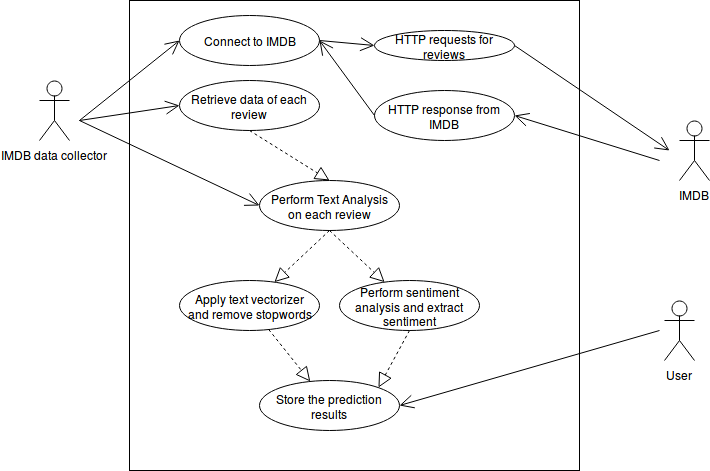
\includegraphics[width=5.2in,height=4.5in]{usecase2.png}
\caption{Use Case : System}
\end{figure}
\newpage
\section{Model and Description}
This section contains details about events and associated behaviour of the system which is shown using diagram below.

\subsection{Activity Diagram}
Activity diagram is a flow chart to represent the flow form one activity to another activity. The activity can be described as an operation of the system. The control flow is drawn from one operation to another. This flow can be sequential, branched or concurrent. The purpose of activity diagrams is to capture the dynamic behaviour of the system.\\\\
\textbf{Description} : As shown in figure 7.2, user downloads movie dataset. This dataset is added for processing using csv import 
library. Documents are preprocessed to remove stopwords and reviews are converted into matrix. Classifiers are trained after feature extraction. This trained classifiers are used on test dataset to classify.
\begin{figure}[h!]
\begin{center}
 

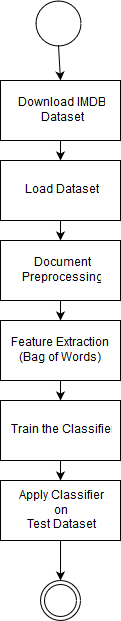
\includegraphics[width=1.0in,height=6.0in]{Activity.png}
\caption{Activity Diagram}
\end{center}

\end{figure}
\newpage
\section{Functional Model and Description}
This section describes data flow diagrams (DFD) of the proposed system. There are three types of DFDs explained in the section. These diagrams explain the system in brief.

\subsection{Data Flow Diagram}
\subsubsection{Level 0 Data Flow Diagram}
In the level 0 DFD as shown in figure 7.3, downloaded reviews are loaded in sentiment analysis system. The sytem analyzes and presents report
through charts to user\\
\begin{figure}[h!]
\begin{center}
 


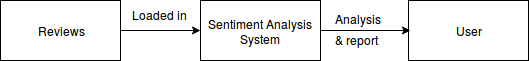
\includegraphics[width=4.5in]{level_0.png}
\caption{Level 0 DFD}
\end{center}
\end{figure}

\subsubsection{Level 1 Data Flow Diagram}
In the level 1 DFD as shown in figure 7.4, Reviews are loaded through csv file loader. Data is preprocessed and model is created.
Analysis done by the system is given to the user.\\
\begin{figure}[h!]
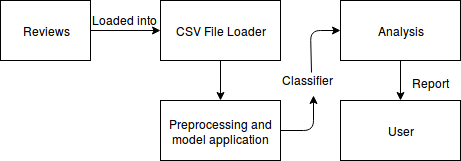
\includegraphics[width=4.5in]{level_1.png}
\caption{Level 1 DFD}
\end{figure}

\subsubsection{Level 2 Data Flow Diagram}
In the level 2 DFD as shown in figure 7.5, Reviews are preprocessed to give bag of words features. Classifiers are trained using this model. Classification is 
performed on the test dataset. Detailed analysis of results obtained by classifiers is done. It is provided to the user.\\
\begin{figure}[h!]
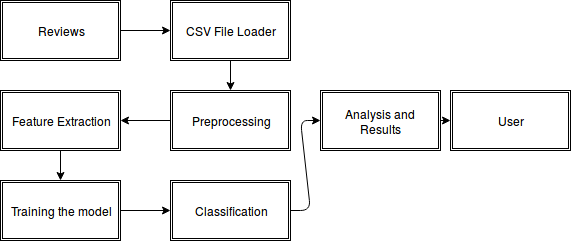
\includegraphics[width=4.5in]{level_2.png}
\caption{Level 2 DFD}
\end{figure}




\section{Non-Functional Requirements}
\subsection{Availability}
Required libraries must be installed and loaded in the python environment with the 
required configurations. Dataset must be downloaded from specified URL \cite{dataset}.

\subsection{Scalability}
The system should be scalable to classify reviews even if the training and test data are increased. System can comfortably handle 
reviews dataset upto 25000 reviews.

\subsection{Performance}
The system must be interactive and delays involved must be less. There should be no immediate delays for every action and response of the system. Training time increases as the training data increases. It takes 4 to 5 seconds in training the dataset. Training increases further when bigram and trigram models are used.


\subsection{Usability}
The system should be easy to handle and process requests efficiently. System's functions are designed to use with ease and provide results. Results are presented in the form of graphs and are easy to comprehend.

\subsection{Reliability}
The system should efficiently analyze movie reviews entirely and give correct classification result. It should be reliable to perform 
classification effectively on any review dataset.
\subsection{Maintainability and Changeability}
The system is made up of different independent modules that can be modified to correct faults, improve performance or other attributes, or adapt to a changed environment. System can be improved for new features and will be able to include new requirements.

\chapter{DETAILED DESIGN DOCUMENT}

\section{Introduction}
This document specifies the design that is used to fetch movie reviews in CSV format, classifies individual movie review into polarity categories.
\begin{itemize}
 


    \item \textbf{Polarity Categories}
    \begin{itemize}
    \item Positive
    \item Negative
   
    \end{itemize}
\end{itemize}
IMDB movie dataset is downloaded and classified using machine learning classifier.
Results obtained by various classifiers are compared with each other.
\newpage
\section{Architectural Design}
Figure 8.1 shows architectural design of proposed system. Following are important components in the system :
\begin{itemize}
\item Movie reviews data : It contains 1,000 positive and 1,000 negative movie reviews from IMDB.
\item Preprocessing : It has stopwords removal and vectorizer.
\item Training data and Test Data : Data is divided into training data and test data. Training data consists of 75\%
of data and test data consists of 25\% of total data. Both are mutually exclusive.
\item Classifier : Training data is given as a input to one of the classifier.
\item Prediction system : It takes test data and applies trained model to it .
\item Sentiment : It stores the end output of polarity into positive and negative classification.   
\end{itemize}

\vspace{5mm}
\begin{figure}[!h]
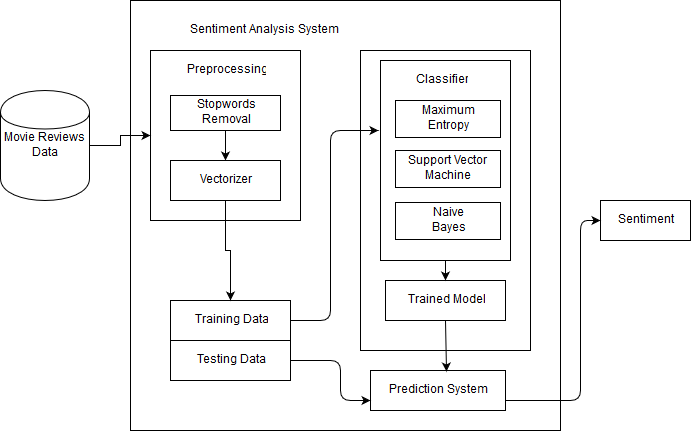
\includegraphics[width=5.0in,height=3.0in]{archi.png}
\caption{Proposed System Architecture}
\end{figure}

\section{Class Design}
It is a static diagram that represents the static view of an application. 
It is not only used for visualizing, describing, and documenting different
aspects of a system but also for constructing executable code of the software 
application. It describes the attributes and operations of a class and also
the constraints imposed on the system.
\\\\
\textbf{Description} : In figure 8.2, modules and their relationships are shown.
Document classifier used for classifying.
SentimentClassification class has ClassifyReview method which predicts the polarity of review.
The fit method in every classifier
converts the text data into matrix of word frequency counts.
\vspace{5mm}
\begin{figure}[h!]
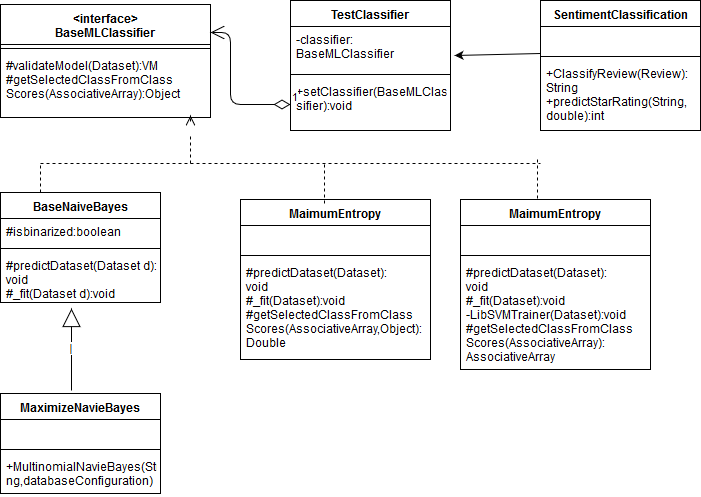
\includegraphics[width=5.5in,height=4.0in]{class.png}
\caption{Class Diagram}
\end{figure}
\newpage
\section{Component Design}
It is used to model the physical aspects of a system. It is also used to visualize the organization and relationships among components in a system. It does not describe the functionality of the system but it describes the components used to make those functionalities.\\\\
\textbf{Description} : Figure 8.3 describes primary components of the system.
Movie dataset is stored in a component which then gives to classifier system.
Classifier system then preprocess the reviews and does the prediction of polority and sends the output
to the console subsystem where result evaluation and comparison takes place.
\begin{figure}[h!]
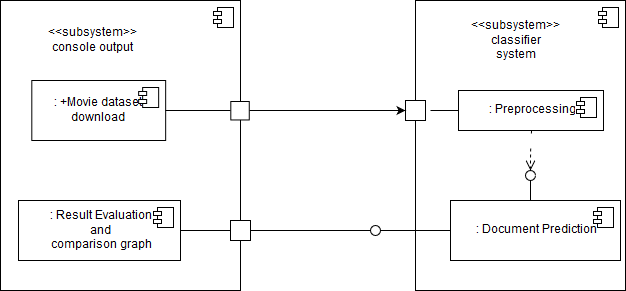
\includegraphics[width=5.2in,height=3.2in]{Component_.png}
\caption{Component Diagram}
\end{figure}

\newpage

\subsection{Sequence Diagram}
A sequence diagram is an interaction diagram that shows how objects operate
with one another and in what order. It is a construct of a message sequence chart.

A sequence diagram shows object interactions arranged in time sequence. 
It depicts the objects and classes involved in the scenario and the sequence
of messages exchanged between the objects needed to carry out the functionality 
of the scenario. Sequence diagrams are typically associated with use case 
realizations in the Logical View of the system under development. 
Sequence diagrams are sometimes called event diagrams or event scenarios.

\textbf{Description} : Training data sends reviews to feature extraction module.
It gives input to the classifier module. Testing data is received by learned classifier which 
returns the opinion type of a particular review.
\vspace{4mm}
\begin{figure}[h!]
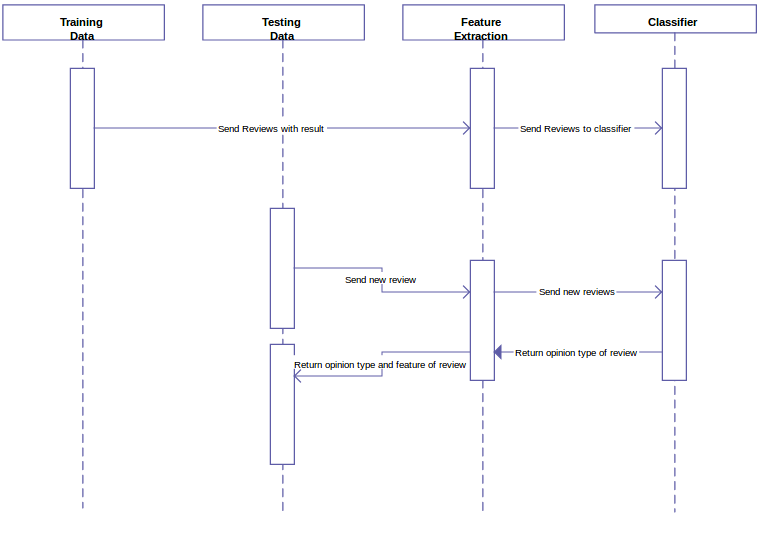
\includegraphics[width=6.0in,height=5.0in]{sequence.png}
\caption{Sequence Diagram}
\end{figure}

\chapter{IMPLEMENTATION DETAILS}
\section{Introduction}
This section describes implementation of the system, required libraries and dependencies needed for components of the system and use of implementation strategy.
\section{Algorithm}
\subsection{Document Classification}



\textbf{Input} : Movie review dataset in .csv file format \\
\textbf{Output} : Polarity classification \\

\begin{enumerate}
\item Initialize review\_data list to empty
\item Initialize review\_label list to empty
\item Read csv file
\item Put first column of each row in csv in review\_data
\item Put second column of each row in csv in review\_label
\item Specify ngram range i.e. unigram, bigram or trigram
\item Fit the review\_data into matrix form using countvectorizer
which stores counts of each word in a review.
\item Transform review\_data to tfidf using tfidftransformer.
\item Split review\_data and review\_label into review\_train, 
label\_train, review\_test and label\_test
\item Give review\_train and label\_train as input to the classifier
and store learned model in classifier variable.
\item Apply review\_test on classifier model with predict method
and take predicted labels output in predicted variable
\item Compare label\_test with predicted vaiable label values
\item Print the confusion matrix
\end{enumerate}\section{Dataset}
\hspace{1.1cm} Pang and Lee's Movie Review Data was one of the first widely-available sentiment analysis datasets.
It contains 1,000 positive and 1,000 negative movie reviews from IMDB. The text is similar to movies reviews on IMDB today.

\par The file movie-pang02.zip contains a copy of Pang and Lee's movie review data in a
csv format that can be imported directly in python. It has two categories: Pos 
(reviews that express a positive or favorable sentiment) and Neg (reviews 
that express a negative or unfavorable sentiment). For this work, we will assume that
all reviews are either positive or negative; there are no neutral reviews. 
\par For document classification, a training and testing dataset is required. 
Training records for polarity categories are mentioned in Table 9.1

\renewcommand{\arraystretch}{1.5}

\begin{table}[h!]
\centering
\caption{Polarity Training Dataset}
\label{my-label}
\begin{tabular}{|l|l|}
\hline
\textbf{Polarity} & \textbf{Training Records} \\ \hline
Positive          & 1000                      \\ \hline
Negative          & 1000                      \\ \hline

\textbf{Total}    & \textbf{2000}             \\ \hline
\end{tabular}
\end{table}

\newpage
\section{Snapshots}


\begin{figure}[!h]
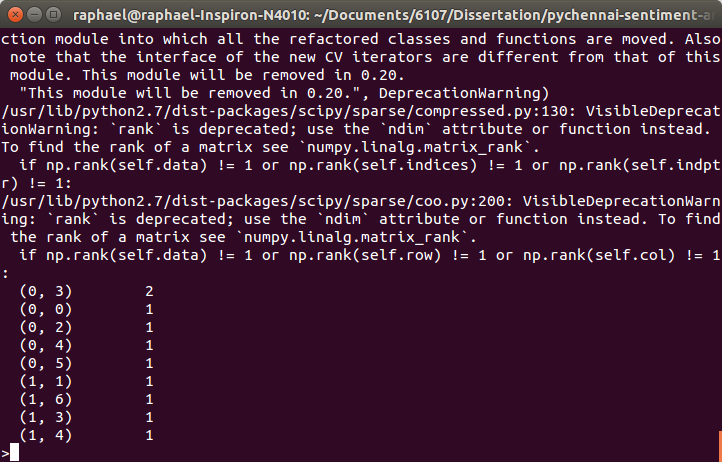
\includegraphics[width=5.5in,height=3.5in]{screenshot2.png}
\caption{Sample Matrix Creation with Word Counts}
\end{figure}

\begin{figure}[!h]
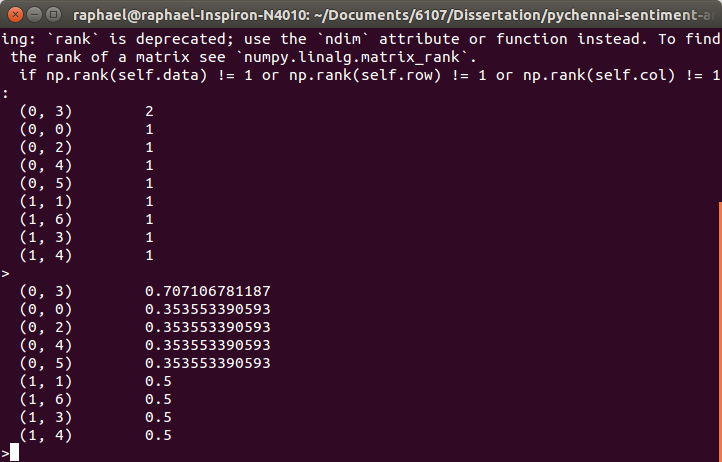
\includegraphics[width=5.5in,height=3.5in]{screenshot3.png}
\caption{Sample Matrix Creation with Tf-idf}
\end{figure}

\begin{figure}[!h]
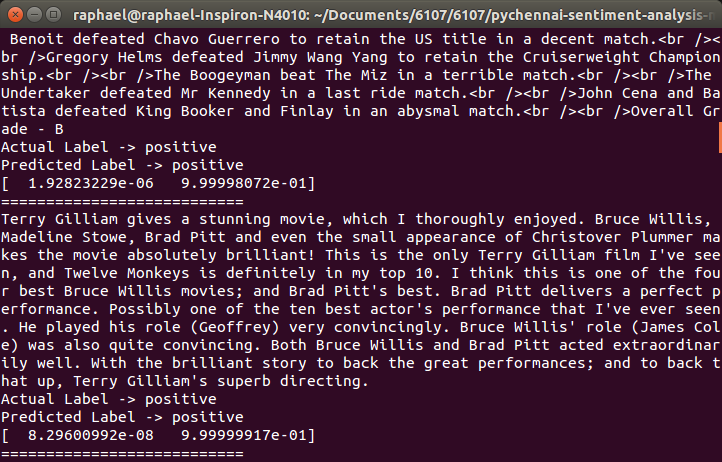
\includegraphics[width=5.5in,height=3.5in]{screenshot1.png}
\caption{Review Classification with Negative and Positive Percentages}
\end{figure}


\begin{figure}[!h]
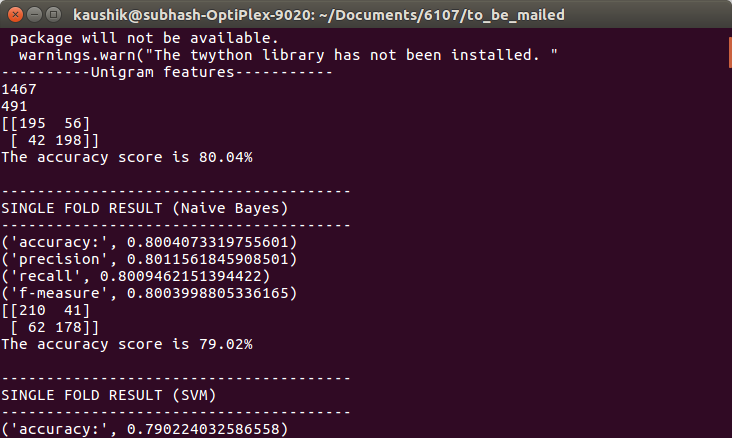
\includegraphics[width=5.5in,height=3.3in]{screenshot4.png}
\caption{Three Classifiers Results (Accuracy, Recall, Precision, F-measure with Confusion Matrix)}
\end{figure}



\begin{figure}[!h]
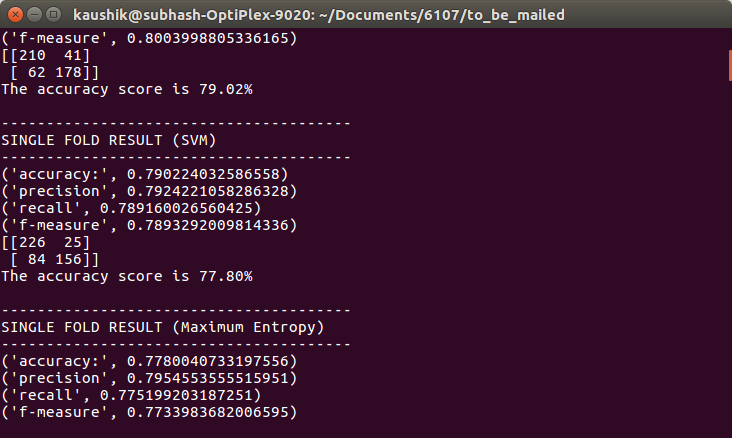
\includegraphics[width=5.5in,height=3.3in]{screenshot5.png}
\caption{Three Classifiers Results (Accuracy, Recall, Precision, F-measure with Confusion Matrix)}
\end{figure}


\begin{figure}[!h]
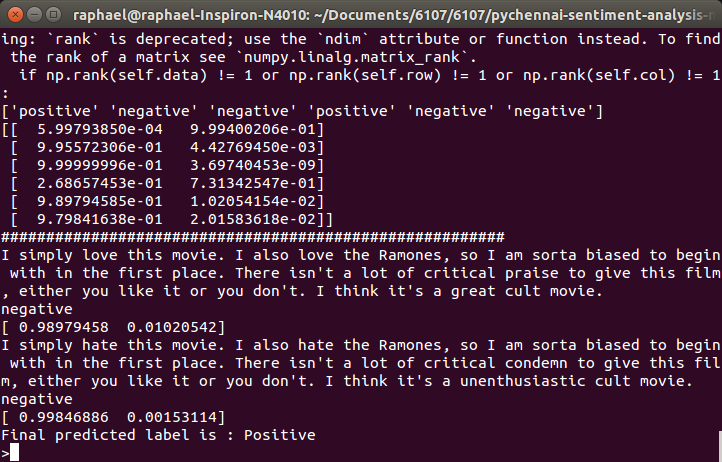
\includegraphics[width=5.5in,height=3.3in]{screenshot_1.png}
\caption{Results of Original and Opposite Reviews}
\end{figure}


\chapter{DATA TABLES AND DISCUSSIONS} 


\section{Result Tables}

\begin{table}[h!]
\centering
\caption{Unigram Features Results}
\label{my-label}
\begin{tabular}{|l|l|l|l|l|}
\hline
\textbf{Classifier} & \textbf{Accuracy} & \textbf{Precision} & \textbf{Recall} & \textbf{F-measure}\\ \hline
Naive Bayes          & 80.04  & 80.11 & 80.09 & 80.03                   \\ \hline
Support Vector Machine          & 79.02  & 79.24 & 78.91 & 78.93                   \\ \hline
Maximum Entropy          & 77.80  & 79.54 & 77.51 & 77.33 \\ \hline
\end{tabular}
\end{table}



\begin{table}[h!]
\centering
\caption{Bigram Features Results}
\label{my-label}
\begin{tabular}{|l|l|l|l|l|}
\hline
\textbf{Classifier} & \textbf{Accuracy} & \textbf{Precision} & \textbf{Recall} & \textbf{F-measure}\\ \hline
Naive Bayes          & 81.26  & 81.43 & 81.34 & 81.25                   \\ \hline
Support Vector Machine          & 80.44  & 80.49 & 80.39 & 80.41                   \\ \hline
Maximum Entropy          & 80.85  & 82.13 & 80.62 & 80.57 \\ \hline
\end{tabular}
\end{table}





\begin{table}[h!]
\centering
\caption{Trigram Features Results}
\label{my-label}
\begin{tabular}{|l|l|l|l|l|}
\hline
\textbf{Classifier} & \textbf{Accuracy} & \textbf{Precision} & \textbf{Recall} & \textbf{F-measure}\\ \hline
Naive Bayes          & 80.85  & 80.90 & 80.90 & 80.85                   \\ \hline
Support Vector Machine          & 80.04  & 80.34 & 79.92 & 79.93                   \\ \hline
Maximum Entropy          & 77.59  & 79.52 & 77.30 & 77.09 \\ \hline
\end{tabular}
\end{table}

\vspace{5mm}
\par The above Table 10.1, Table 10.2, Table 10.3 shows accuracy, precision, recall and F-measure
of three different classifiers. Three different features are used as features.
First table shows results with unigram features i.e. each words is considered separate features.
Second table shows results with bigram features i.e. 2 words together are considered as features.
Third table shows results with trigram features i.e. 3 words combine are considered as features.
\newpage
\section{Result Graphs}
\vspace{5mm}

\par Below fig. 10.1 shows comparison of accuracy scores shown in Table 10.1, Table 10.2, Table 10.3 .

\begin{figure}[!h]
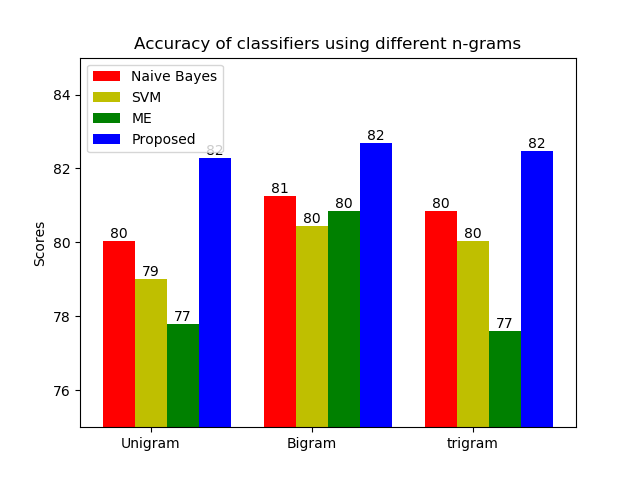
\includegraphics[width=5.0in,height=4.0in]{Comparison.png}
\caption{Classifiers Accuracy Score Comparison}
\end{figure}


\begin{figure}[!h]
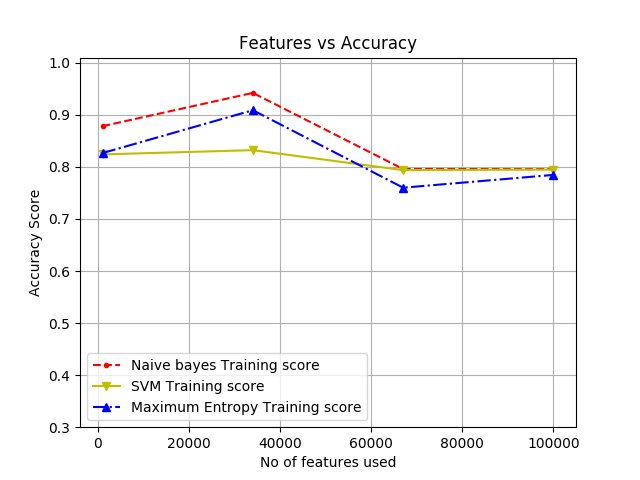
\includegraphics[width=5.0in,height=4.0in]{figure_1.png}
\caption{Variations in Classifier Accuracies as the no. of Features Increases}
\end{figure}



\chapter{CONCLUSION}
In this work, the dual sentiment analysis technique is used
to address the polarity shift problem in sentiment classification.
The idea behind this is to create opposite reviews of the
original reviews and used them together in bag of words model
which will be the feature inputs to various machine learning
algorithms such as Naive Bayes, SVM and Maximum Entropy. It
performs better than the methods which were used to address
the problem of polarity shift due to negation .

\chapter{FUTURE ENHANCEMENTS} 
The research can be extended to include the neutral reviews as well.
Also antonym can be obtained using words that has opposite polarity in the corpus.
This corpus-based pseudo-antonym dictionary is also good at obtaining
more domain-relevant antonym words by learning from the
corpus.


\begin{thebibliography}{20}



\bibitem{xiaOriginal}R. Xia, F. Xu, C. Zong, Q. Li, Y. Qi and T. Li, `` Dual sentiment analysis: Considering  two  sides  of  one 
review, '' in {\em IEEE transactions on knowledge and data engineering,} vol. 27, no. 8, pp. 2120
-
2133, 2015.

  \bibitem{yahoo}S. Das and M. Chen, `` Yahoo! for Amazon: Sentiment extraction from small talk on the web, '' {\em Management science} , Vol.53, Issue no.9, pp. 1375-1388, 2007.

  
  
  \bibitem{pang}Pang, L. Lee, and S. Vaithyanathan, `` Thumbs up? : Sentiment classification using machine
  learning techniques, ''{\em Proceedings of the ACL-02 conference on Empirical methods in natural language processing,}
  pp. 79-86, 2002.
  
  \bibitem{pang2008}B. Pang and L. Lee, `` Opinion mining and sentiment analysis, '' {\em Foundations
  and Trends in Information Retrieval,} vol. 2, no. 1-2, pp. 1-135, 2008.
  
  \bibitem{xia}R. Xia, T. Wang, X. Hu, S. Li, and C. Zong, `` Dual Training and Dual
Prediction for Polarity Classification,'' {\em Proceedings of the Annual 
Meeting of the Association for Computational Linguistics (ACL - 02)} pp. 521-525,
2013.
  \bibitem{turney}P. Turney, `` Thumbs up or thumbs down? Semantic orientation applied to 
  unsupervised classification of reviews, '' Proceedings of the Annual Meeting of 
  the Association for Computational Linguistics (ACL), pp. 417-424, 2002.

  
  \bibitem{contrast}M. Li and C. Huang, `` Sentiment classification considering negation
and contrast transition, '' {\em Proceedings of the Pacific Asia Conference on
Language, Information and Computation (PACLIC),}  pp. 307-316, 2009.


  \bibitem{Shift}Li, S. Lee, Y. Chen, C. Huang and G. Zhou, `` Sentiment 
  Classification and Polarity Shifting, '' {\em Proceedings of the International Conference on
  Computational Linguistics (COLING),} pp. 635-643, 2010.
  
 
  
  \bibitem{turney1}D. Turney and Michael L. Littman, `` Un-supervised learning of semantic orientation from
a hundred-billion-word corpus, '' {\em Technical Report
EGB-1094, National Research Council Canada,} arXiv preprint cs/0212012, 2002.

  \bibitem{vector}Yuan Wang, Zhaohui Li, Jie Liu, Zhicheng He, Yalou Huang and Dong Li,
 `` Word Vector Modeling for Sentiment Analysis
of Product Reviews, '' {\em Natural Language Processing and Chinese Computing 2014,} pp. 168-180, 2014.
 
 \bibitem{base} A Tripathy, A Agrawal, SK Rath , ``Classification of sentiment reviews using 
n-gram machine learning approach, '' in {\em Expert Systems with Applications}
Volume 57, pp. 117-126, 2016.

\bibitem{salvetti} Salvetti, Franco, Stephen Lewis, and Christoph Reichenbach. 
``Automatic opinion polarity classification of movie,'' {\em Colorado research in linguistics 17,} no. 2 2004.

\bibitem{xiaco}Xia, Rui and Wang, Cheng and Dai, Xinyu and Li, Tao, 
`` Co-training for Semi-supervised Sentiment Classification Based on Dual-view Bags-of-words Representation, ''
  {\em Association for Computational Linguistics (ACL 1),} pp. 1054-1063, 2015.
  
\bibitem{na}Na, J.C., Sui, H., Khoo, C., Chan, S., and Zhou, Y., `` Effectiveness of Simple Linguistic 
Processing in Automatic 
Sentiment Classification of Product Reviews, '' {\em Proceedings 
of the Eighth International ISKO Conference
 } pp. 49-54, 2004.
 
 \bibitem{rui22}Rui Xia, Feng Xu, Jianfei Yu, Yong Qi and Erik Cambria, `` Polarity shift detection, 
 elimination and ensemble:
A three-stage model for document-level sentiment analysis, '' {\em  Information Processing \& Management 
52, no. 1, } pp. 36 - 45, 2016

\bibitem{ruiEnssemble}Rui Xia, Chengqing Zong and Shoushan Li, `` Ensemble of feature sets and classification algorithms
for sentiment classification, '' {\em  Information Sciences 181, no. 6 } pp. 1138-1152, 2011

\bibitem{Kauer}Anderson Uilian Kauer and Viviane P. Moreira, `` Information retrieval for sentiment polarity prediction, ''
{\em Expert Systems With Applications 61,} pp. 282 - 289, 2016

\bibitem{Theory}Yuming Lin, Jingwei Zhang, Xiaoling Wang and Aoying Zhou, `` An Information Theoretic 
Approach to Sentiment Polarity
Classification, '' {\em Proceedings of the 2nd joint WICOW/AIRWeb workshop on web quality, 
ACM Lyon France }, pp. 35 - 40, 2012


\bibitem{valence}L. Polanyi and A. Zaenen, `` Contextual lexical valence shifters, '' in
{\em Proc. AAAI Spring Symp. Exploring Attitude Affect Text}, pp. 1–10, 2004.

\bibitem{dataset}http://boston.lti.cs.cmu.edu/classes/95-865-K/HW/HW3/movie-pang02.zip
\end{thebibliography}

\appendix
\chapter{PAPERS PUBLISHED}
\section{Paper Title}
Sentiment Analysis using Machine Learning Algorithms: A Survey
\subsection{IJIRCCE Certification}
\begin{figure}[!h]

\includegraphics[width=5.7in,height=4.7in]{ijircce.png}
\caption{IJIRCCE Certificate}
\end{figure}
\section{Paper Title}
Sentiment Analysis using Original and Reversed Reviews
\newpage
\subsection{cPGCON Certificate}

\begin{figure}[!h]

\includegraphics[width=5.5in,height=4.2in]{6107_certificate.jpg}
\caption{cPGCON Certificate}
\end{figure}

\newpage
\subsection{cPGCON Review}
\begin{figure}[!h]
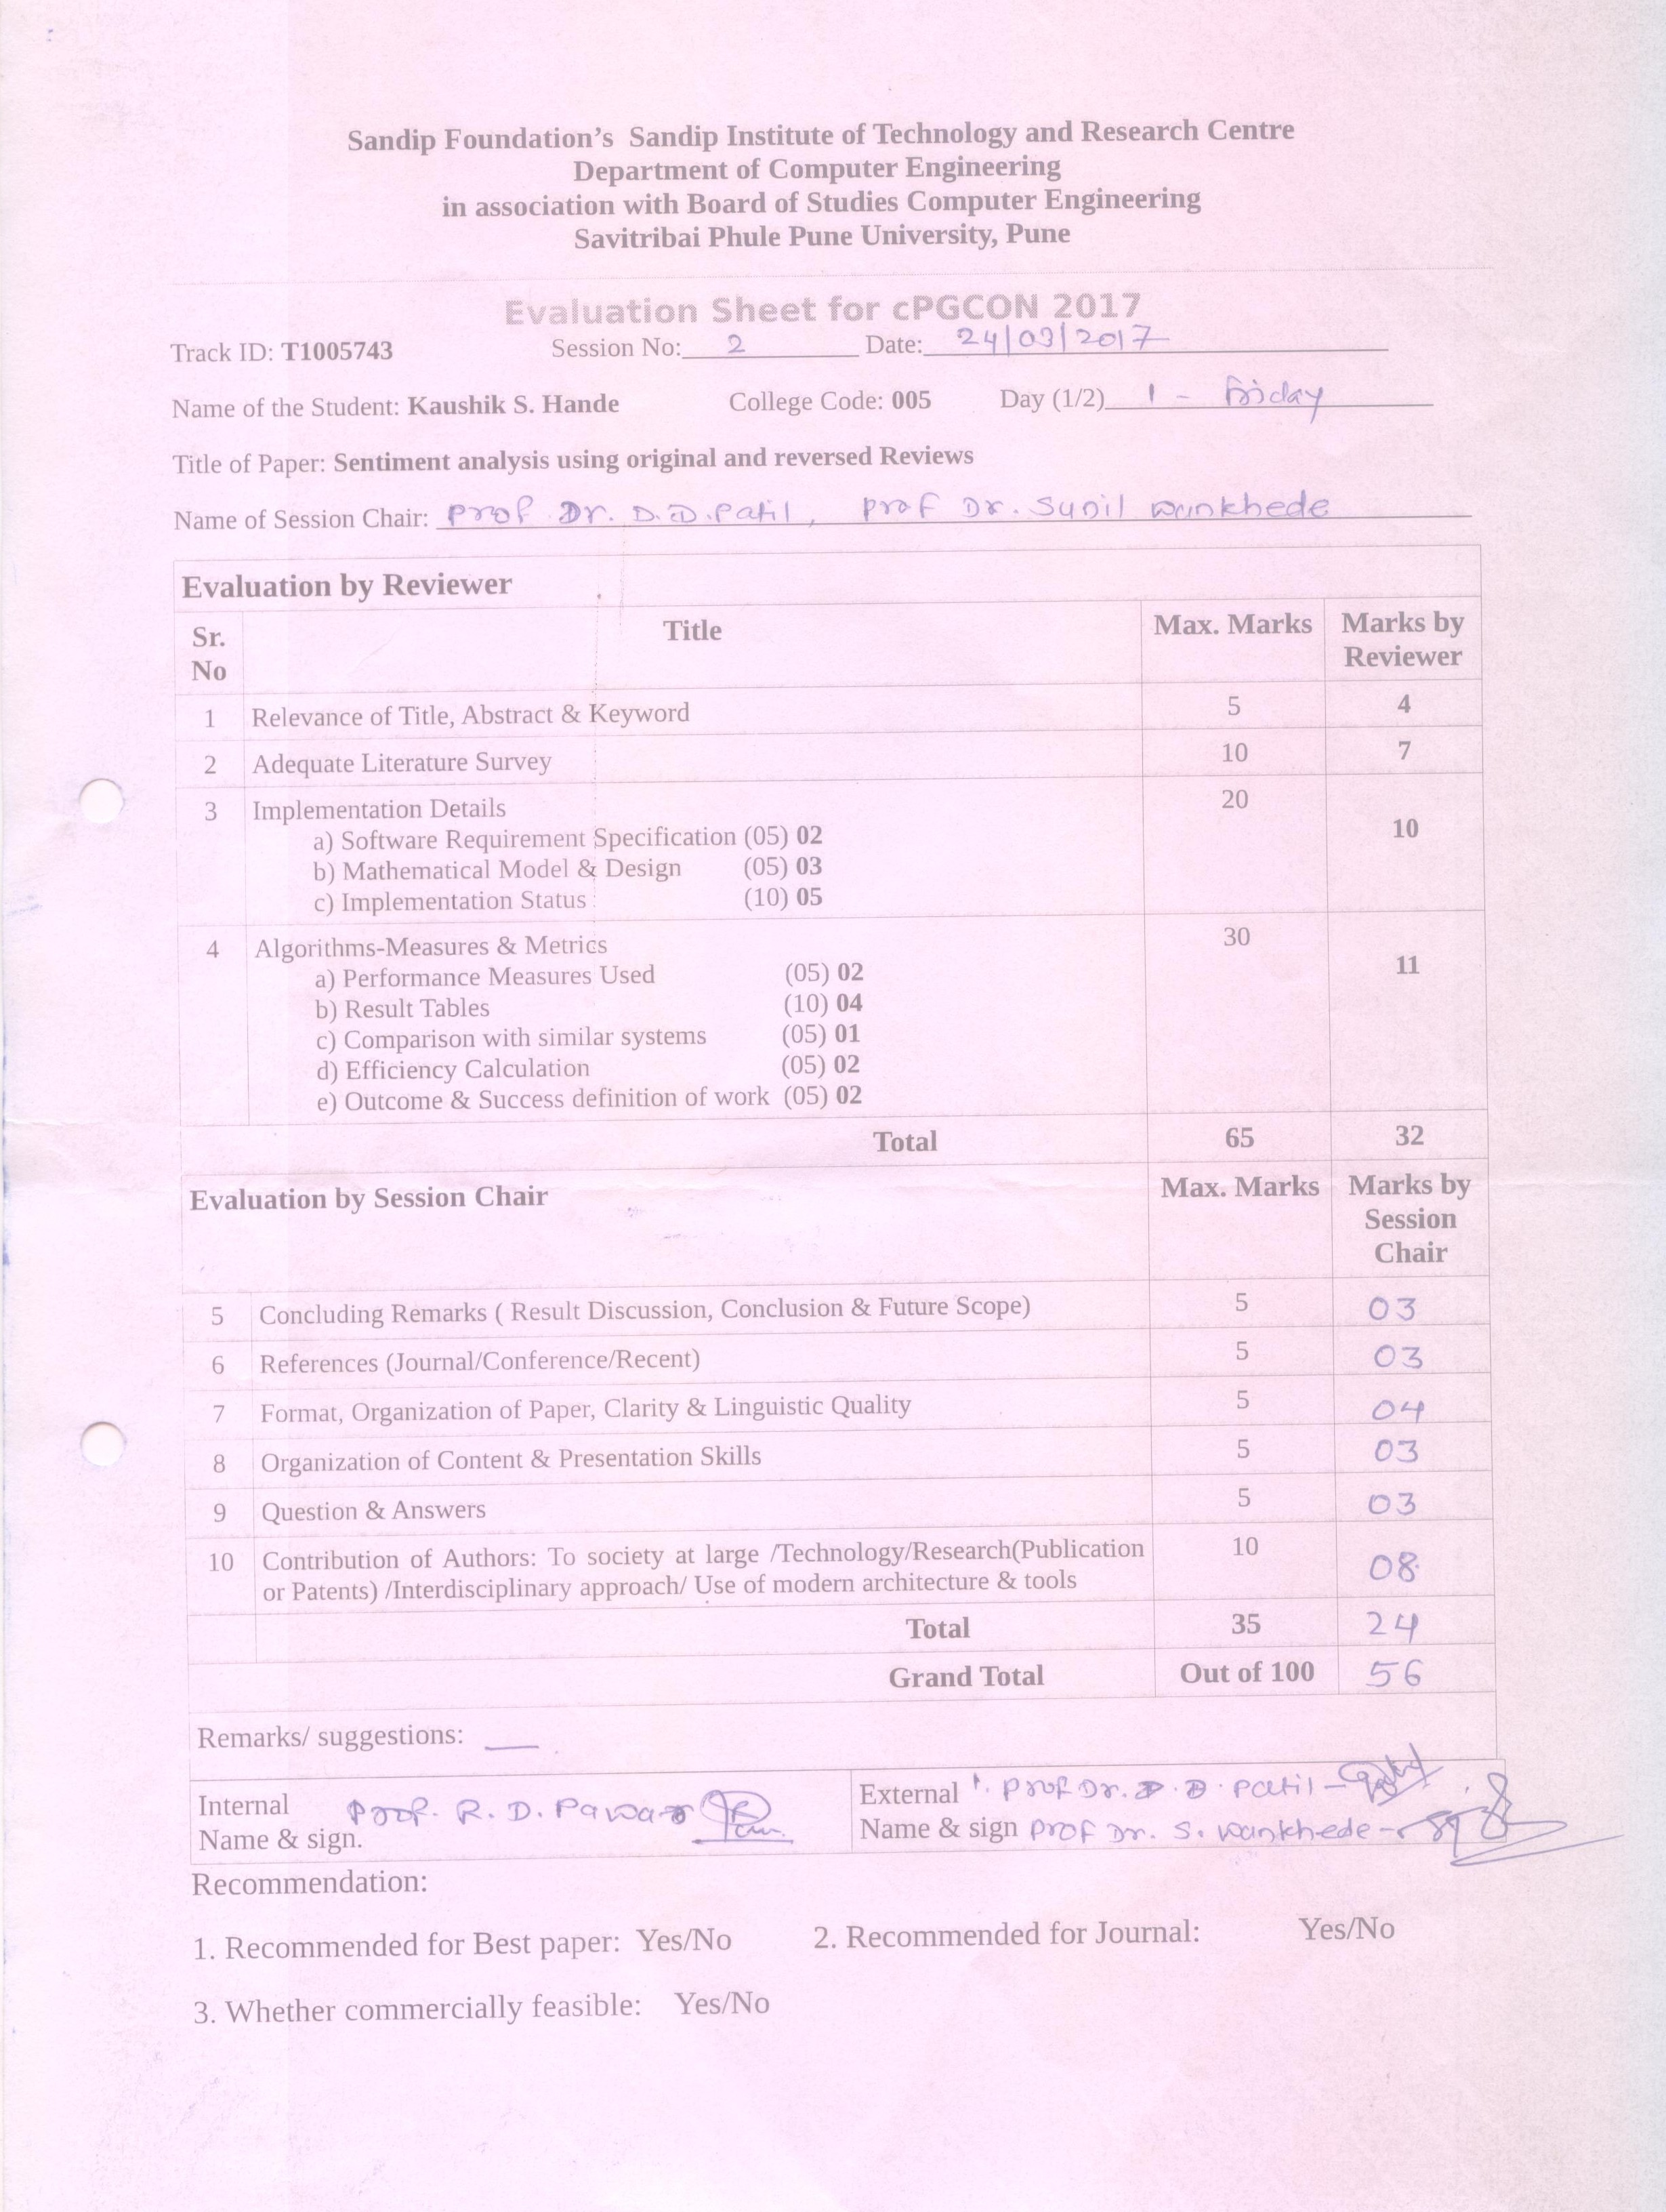
\includegraphics[width=5.5in,height=7.2in]{6107_reviewsheet.jpg}
\caption{cPGCON Review Sheet}
\end{figure}

\chapter{DISSERTATION PLANNER}
\renewcommand{\arraystretch}{1.5}
\begin{table}[]
\centering
\caption{Dissertation Task Set}
\label{my-label}
\begin{tabular}{|l|l|}
\hline
\textbf{Task Title} & \textbf{Dissertation Task}                    \\ \hline
T1                  & Study of Domain - Machine Learning and Natural Language Processing         \\ \hline
T2                  & Identification of problem in existing systems \\ \hline
T3                  & Review of literature \\ 
\hline
T4                  & Building mathematical model \\ 
\hline
T5                  & Report on scheme of implementation \\ \hline
T6                  & Identification of prerequisites and installation \\ \hline
T7                  & Configuring python and python package installer pip in the system \\ \hline
T8                  & Study of various machine learning algorithms and its implementation in python\\ \hline
T9                  & Studying libraries in python required for implementation \\ \hline
T10                  & Downloading and extracting reviews from IMDB movie datasets \\ \hline
T11                  & Removing stopwords, punctuation marks, numbers etc.\\ \hline
T12                  & Report preparation \\ \hline
T13                  & Dissertation project stage I presentation \\ \hline
T14                  & Document preprocessing
 \\ \hline
T15                  & Creating bag of words model from movie reviews.
 \\ \hline
T16                  & Spliting the dataset into training and test dataset \\ \hline
T17                  & Train machine learning classifiers using bag of words model.\\ \hline
T18                  & Create unigram, bigram, trigram variations of model \\ \hline
T19                  & Train machine learning classifiers using this model.
 \\ \hline
T20                  & cPGCON paper presentation
 \\ \hline
T21                  & Predictive model construction \\ \hline
T22                  & Model testing \\ \hline
T23                  & Experimental results, analysis and validation of results \\ \hline
T24                  & Project review with demonstration
 \\ \hline
T25                  &Report Validation 
 \\ \hline
 T26                  &Report Submission
 \\ \hline

\end{tabular}
\end{table}
\end{document}
